
\chapter{LEGO MINDSTORMS NXT}
I dette kapitel vil den valgte platform, \legoms, blive kort beskrevet, samt en begrundelse for dette valg.
Yderligere vil der blive argumenteret for valg af API til NXT-enheden.

\section{Hvad er LEGO MINDSTORMS?}
\legoms er et byggesæt, hvor det er muligt at bygge programmerbare robotter(her menes også andre maskiner der måske ikke altid vil blive betegnet som robotter) i \lego-klodser.

Til at bygge disse robotter er der i \legoms nogle sensorer og aktuatorer. Sensorerne gør det muligt for robotten at modtage input fra sine omgivelser og ved brug af aktuatorerne kan robotten reagere på disse.

Ud over de originale \lego dele er der også tredjeparts forhandlere, som har et udbud af andre sensorer og aktuatorer.

\subsection{Hvad er NXT?}
Denne sektion er baseret på \cite{nxt}.
NXT Intelligent Brick (oftest kaldt blot 'NXT' eller 'brick') er hjernen i \legoms robotten.
Det er den der står for at modtage og behandle input fra sensorer, samt at styre aktuatorer.
Et billede af NXT'en kan ses i \cref{platform:nxt}.

\begin{figure}
\begin{center}
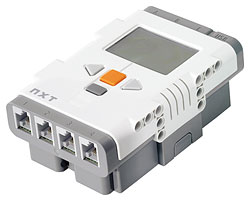
\includegraphics[scale=1]{./graphics/nxt/nxt}
\end{center}
\caption{'NXT Intelligent Brick'}
\label{platform:nxt}
\end{figure}

\paragraph{Porte}
NXT'en har 3 motor porte og 4 sensor porte.

\paragraph{Tilslutningsmuligheder}
Der kan kommunikeres med NXT'en enten ved at tilslutte den med USB-kabel eller ved Bluetooth\textregistered.

\paragraph{Feedback}
Til output har NXT'en en 100 x 64 pixel LCD display samt 8 kHz højttaler.

\paragraph{Styring}
NXT'en kan styres på to måder:
Man kan sende kommandoer og modtage beskeder (for eksempel sensor aflæsninger) på en ekstern enhed (oftest en computer eller en anden NXT).
Alternativt kan programmer sendes (via Bluetooth eller USB) til NXT'en, hvorfra de kan køres direkte på NXT'en, uafhængig af eksterne enheder.

Til at styre NXT'en kan bruges et væld af programmeringssprog.
Yderligere er det også muligt at erstatte den originale firmware med en brugerdefineret, hvilket giver endnu flere muligheder.
Kombination af firmware og programmeringssprog (samt eventuelle værktøjer) er hvad vi betragter som et API.
De forskellige API'er samt vores valg af API diskuteres i \cref{nxt_api}.

\paragraph{Tekniske specifikationer}
De tekniske specifikationer for NXT'en:\cite{nxt}
\begin{itemize}
\item{32-bit ARM7 microcontroller}
\item{256 Kb FLASH, 64 Kb RAM}
\item{8-bit AVR controller}
\item{4 Kb FLASH, 512 b RAM}
\item{Bluetooth wireless communication (Bluetooth Class II V2.0 compliant)}
\item{USB full speed port (12 Mbit/s)}
\item{4 input ports, 6-wire cable digital platform (One port includes a IEC 61158 Type 4/EN 50 170 compliant expansion port for future use)}
\item{3 output ports, 6-wire cable digital platform}
\item{100 x 64 pixel LCD graphical display}
\item{Loudspeaker - 8 kHz sound quality. Sound channel with 8-bit resolution and 2-16 kHz sample rate}
\item{Power source: 6 AA batteries}
\end{itemize}

\section{Hvorfor LEGO MINDSTORMS NXT?}
Der er mange gode grunde til at vælge \legoms NXT.
Her er givet fire overordnede punkter, der vil blive gennemgået efterfølgende:

\begin{itemize}
\item{Tilgængelighed}
\item{Nemt at gå til}
\item{Stort udvalg af sensorer}
\item{Mange muligheder ift. styring}
\end{itemize}

\paragraph{Tilgængelighed}
Grundet at \lego (inkl. \legoms) er ment til almindelige brugere, er det masseproduceret og kan derved købes forholdsvist billigt og i helt almindelige butikker (legetøjsforretninger og ofte også supermarkeder).

\paragraph{Nemt at gå til}
Det faktum at man bygger sin robot i \lego klodser, med tilføjelse af \legoms sensorer/aktuatorer, gør at det i første gang er nemt at lave en konstruktion.
Samtidig er det også nemt at tilpasse en tidligere konstruktion, ved at tilføje/ændre/fjerne klodser eller sensorer/aktuatorer.

Denne høje versatilitet gør at \lego er perfekt til en prototype-orienteret fremgangsmåde.

\paragraph{Stort udvalg af sensorer}
Det store udvalg af sensorer gør at der kan bygges robotter der kan løse et væld af opgaver.
Ved et projekt med høj usikkerhed, er det derved også nemt og billigt at udskifte en sensor med en mere passende.

\paragraph{Mange muligheder ift. styring}
Her menes der både overordnet den måde hvorpå robotten styres, men især også den måde hvorpå NXT'en styres.
Som nævnt tidligere kan NXT'en udstyres med brugerdefineret firmware, der gør at der er utroligt få begrænsninger ift. styring af den.
Desuden kan der kommunikeres med NXT'en via et væld af programmeringssprog.
Der vil blive gået mere i dybden med de forskellige muligheder ift. API i \cref{nxt_api}.


\section{Valg af NXT API}
\label{nxt_api}

\subsection{De forskellige API'er}

\subsection{Vores valg}
